\documentclass[10pt, reqno]{article}
\usepackage[utf8]{inputenc}
\usepackage[margin = 1cm, a6paper, landscape]{geometry}
\usepackage{amsmath, amsfonts, amssymb, amsthm, graphicx}
\usepackage[ruled]{algorithm2e}
\usepackage{caption}

\usepackage{hyperref}
\usepackage[dvipsnames]{xcolor}
\hypersetup{colorlinks, linkcolor={MidnightBlue}, citecolor={MidnightBlue}, urlcolor={MidnightBlue}}

\usepackage{tikz}

\setlength{\parindent}{0pt}
\newcommand{\forceindent}{\leavevmode{\parindent=1em\indent}}
\numberwithin{equation}{section}

\newtheorem*{theorem*}{Theorem}
\newtheorem*{cor*}{Corollary}

\newcommand{\norm}[1]{\left\lVert#1\right\rVert}
\newcommand{\e}{\epsilon}
\newcommand{\w}{\omega}
\newcommand{\R}{\mathbb{R}}
\newcommand{\N}{\mathbb{N}}
\newcommand{\Q}{\mathbb{Q}}
\newcommand{\Z}{\mathbb{Z}}
\renewcommand{\ae}[1]{\text{ \hspace{5pt} a.e. #1}}

\begin{document}
%\pagestyle{empty}
\setlength{\footskip}{-1cm}
 

\title{Combining $l^1$ Penalization with Higher Moment Constraints in Regression Models}
\author{Austin David Brown}
\date{\today}

%%%
% Slide
%%%
\maketitle

%%%
% Slide
%%%
\newpage
\section*{Motivation}

\begin{itemize}

\item In statistics and probability theory it is common to impose moment assumptions on a random variable $X : \Omega \to \R^n$ such as $E(\norm{X}^k) < \infty$ for $k \in \R$.

\item These constraints correspond to the $L^p$ spaces which allow control over the width and the height of such random variables.
Thus, these norms give us some "statistics" about the random variable.

\item If statisticians so freely impose such constraints then we should build a tool to allow scientists and researchers to impose similar constraints on their real problems.

\item  In this project, I built an R package to expand upon the idea of ElasticNet \cite{elasticnet}, which I think approximately encapsulates this idea.

\end{itemize}

%%%
% Slide
%%%
\newpage
\section*{Geometric Motivation}
Consider for example an Elasticnet \cite{elasticnet} penalty $Q(x) = \frac{1}{2} |x| + \frac{1}{2} |y| + \frac{1}{2} |x|^2 + \frac{1}{2} |y|^2 \le 1$
shown on the left. Extending this idea, a new penalty $P(x) = \frac{1}{2} |x| + \frac{1}{2} |y| + \frac{1}{2} |x|^4 + \frac{1}{2} |y|^4 \le 1$ shown on the right.

\vspace{.5cm}
\begin{center}
\begin{minipage}{.5\textwidth}
  \centering
  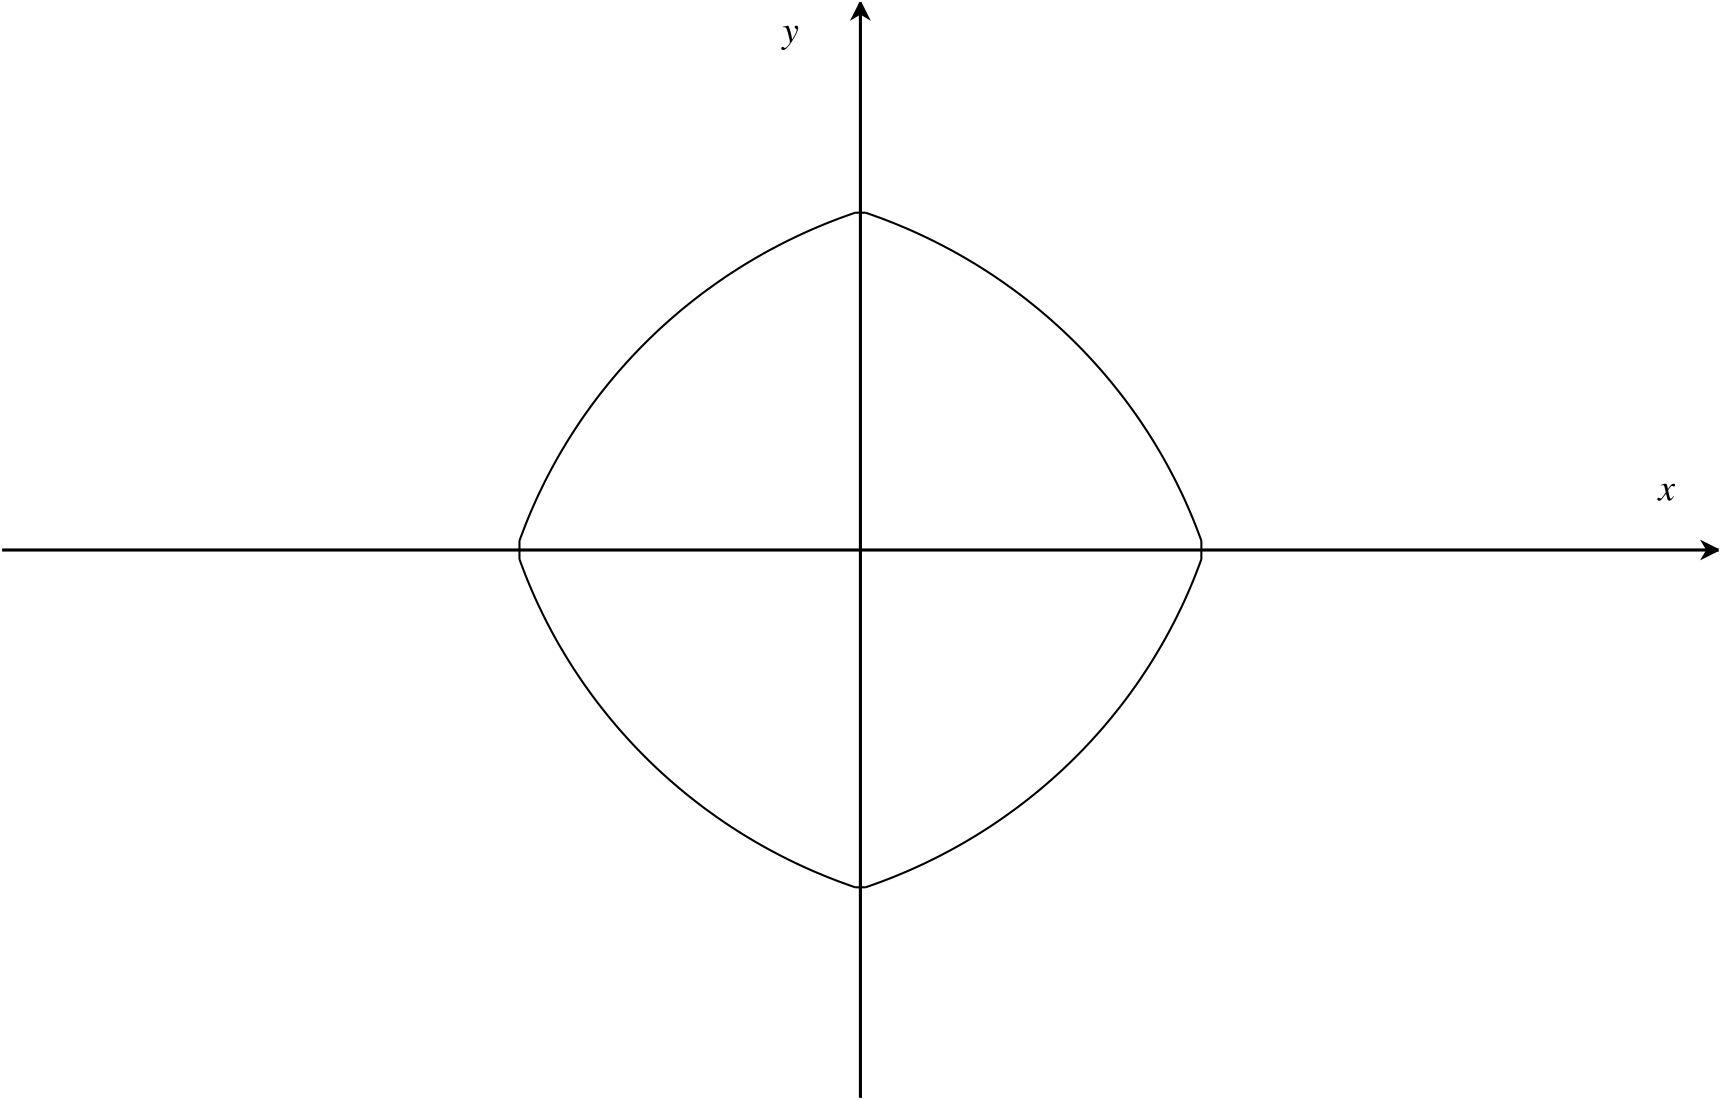
\includegraphics[width=.9\linewidth]{elasticnet.png}
\end{minipage}%
\begin{minipage}{.5\textwidth}
  \centering
  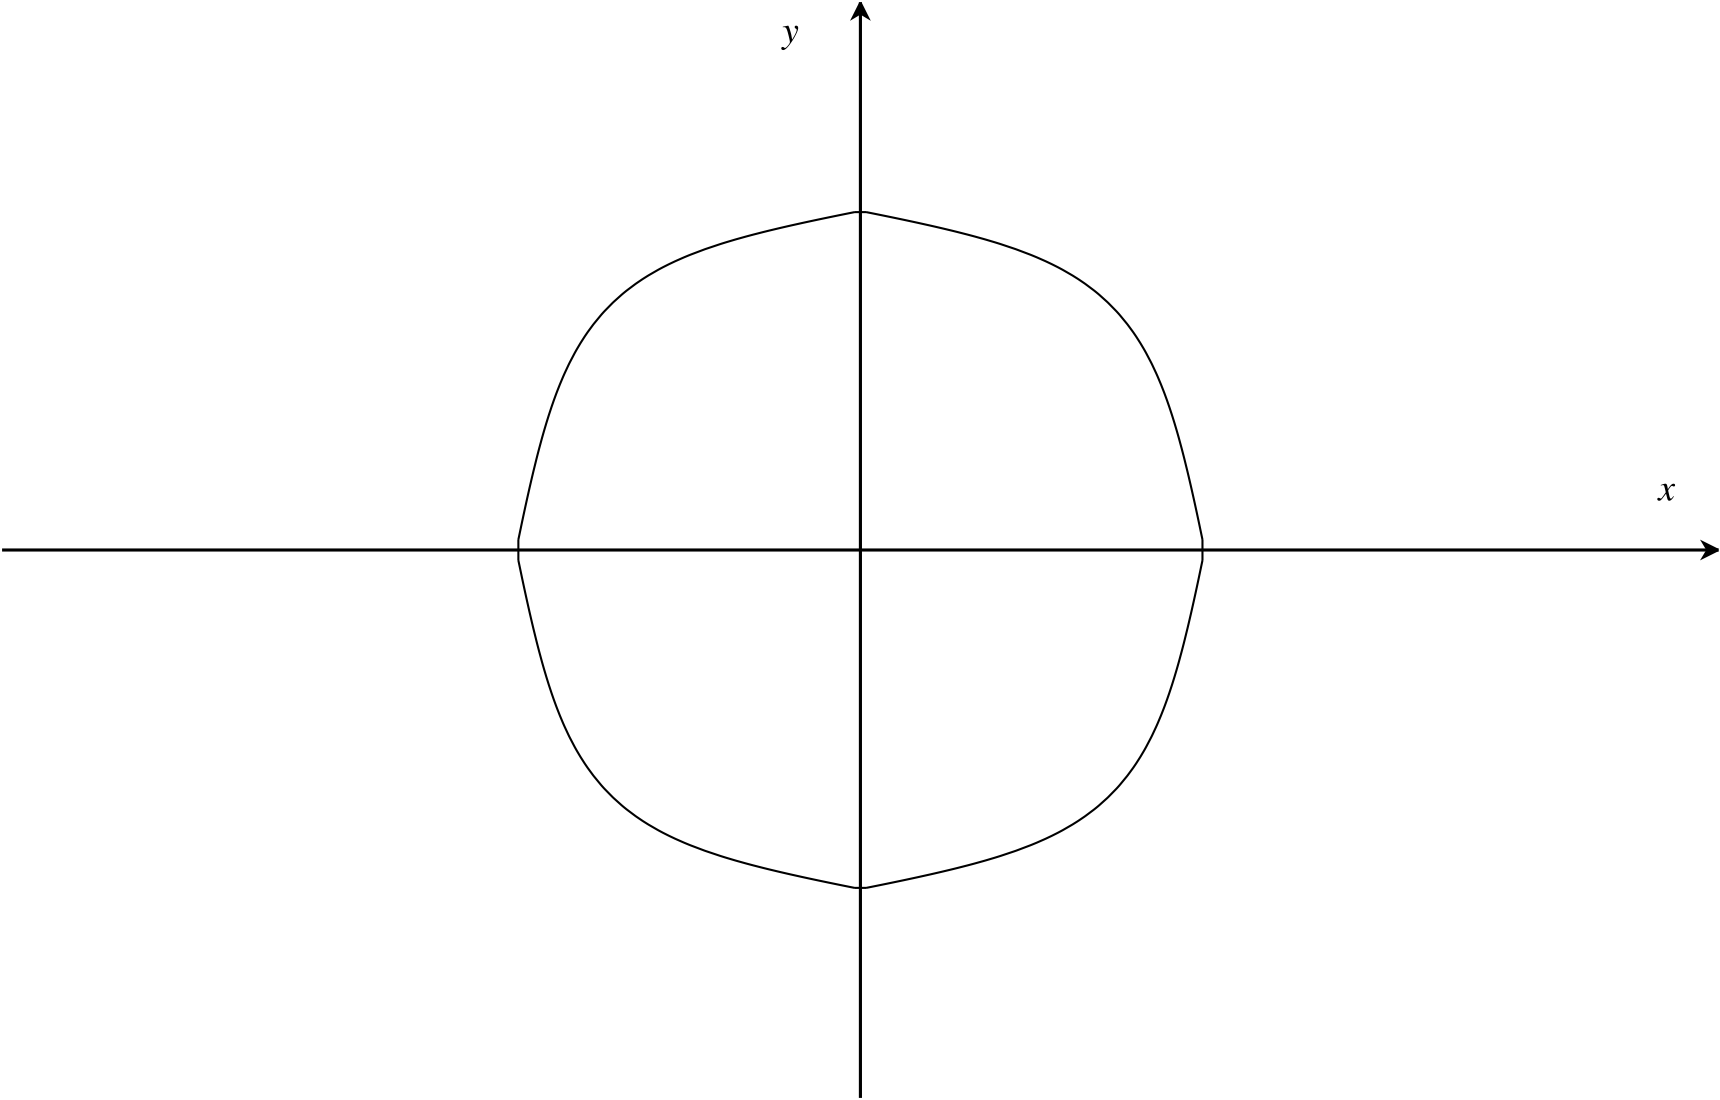
\includegraphics[width=.9\linewidth]{new_penalty_4_moment.png}
\end{minipage}
\end{center}
\vspace{.5cm}

It is possible that a scientist or researcher may want the option to "bow" out the feasible set even more or maybe Elasticnet \cite{elasticnet} excludes a good solution.

%%%
% Slide
%%%
\newpage
\section*{The Setup}

Define a new penalty to try to impose more "stability" for scientists and researchers (try to extend the Elasticnet \cite{elasticnet} idea). Let
\[
L_{\lambda}(\beta) = \frac{1}{2} \norm{y - X \beta}_2^2 + \lambda P(\beta)
\]

with penalty

\[
\lambda P(\beta) = \lambda \alpha_0 \norm{\beta}_1 + \lambda \sum_{k = 1}^{5} \alpha_k \norm{\beta}_{2k}^{2k} 
\]

where $y \in \R^n$, $X \in M_{n \times p}(\R)$, and $\beta \in \R^p$, $\lambda \in \R_{+}$ and $\alpha$'s are convex combinations or use separate tuning parameters instead.

\vspace{1cm}
An important property is that this is a convex and completely separable penalty. This allows us to use coordinate descent.

%%%
% Slide
%%%
\newpage
\section*{Algorithm Implementation 1}

\vspace{.5cm}
\begin{algorithm}[H]
\caption{Subgradient Coordinate Method}
Choose $\beta^0 \in \R^p$ and tolerance $\delta > 0$;

Set $k \gets 0$

\Repeat{Until the loss difference $\Delta L$ is less than $\delta$}{ 

  Randomly choose $i_k \in \{1, \ldots, p\}$

  $h_i^k \gets \frac{R}{\sqrt{1 + k}}$ for some $R > 0$ or use $\frac{R}{\sqrt{1 + N}}$ where $N$ is the length of the algorithm.

  $\beta_{i_{k + 1}} \gets \beta_{i_k} - h^k g^{i_k}$ where $g^{i_k} \in (\partial L)_{i_k}$

  $k \gets k + 1$
}

\end{algorithm}

%%%
% Slide
%%%
\newpage
\section*{Drawbacks}

\begin{itemize}
\item Not a descent method, so you cannot do line search.

\item No good stopping criterion.

\item There are many choices for the subgradient.

\item Tends to produce really small values instead of truly sparse solutions.

\end{itemize}

%%%
% Slide
%%%
\newpage
\section*{A Better Algorithm}

\vspace{.5cm}
\begin{algorithm}[H]
\caption{Proximal Gradient Coordinate Descent}
Choose $\beta^0 \in \R^p$ and tolerance $\delta > 0$;

Set $k \gets 0$

\Repeat{Until the Moreau-Yoshida mapping $M_{h_k, f} < \delta$}{ 

  Set the step size $h^k > 0$ constant, diminishing or by line search.

  Randomly choose $i_k \in \{1, \ldots, p\}$

  $\beta^{k + 1}_i \gets (\textbf{prox}_{h^k L})_i ( \beta^k_i - h^k \langle X_i, y - X \beta \rangle )$

  $k \gets k + 1$
}
\end{algorithm}

%%%
% Slide
%%%
\newpage
\section*{Benefits}

\begin{itemize}
\item A descent method, so line search can be implemented.

\item Can be accelerated.

\item Good stopping criterion at approximately $O(p)$ flops.

\item Convergence theory is unchanged from differentiable functions.

\item Coordinate descent theory for differentiable functions is still being actively developed.

\end{itemize}

%%%
% Slide
%%%
\newpage
\section*{Cross-Validation Implementation}

\vspace{.5cm}
\begin{algorithm}[H]
\caption{Warm Start Cross-Validation}
Choose a sequence of Langrangian dual variables $\lambda_1, \ldots, \lambda_N$, and initial value $\beta^0$.

Order $\lambda_{(1)}, \ldots, \lambda_{(N)}$ descending.

$\beta^{Warm} \gets \beta^0$ 

\For{$k \in 1, \ldots, N$}{

  $\beta^k \gets$ Using Cross-Validation with $\lambda_{(k)}$ warm started with $\beta^{Warm}$.

  $\beta^{Warm} \gets \beta^k$
}

\end{algorithm}

%%%
% Slide
%%%
\newpage
\section*{Package Architecture}

Written entirely in C++ for speed and uses Eigen \cite{eigen} for linear algebra. It can be interfaced to many other popular languages.

\vspace{.5cm}
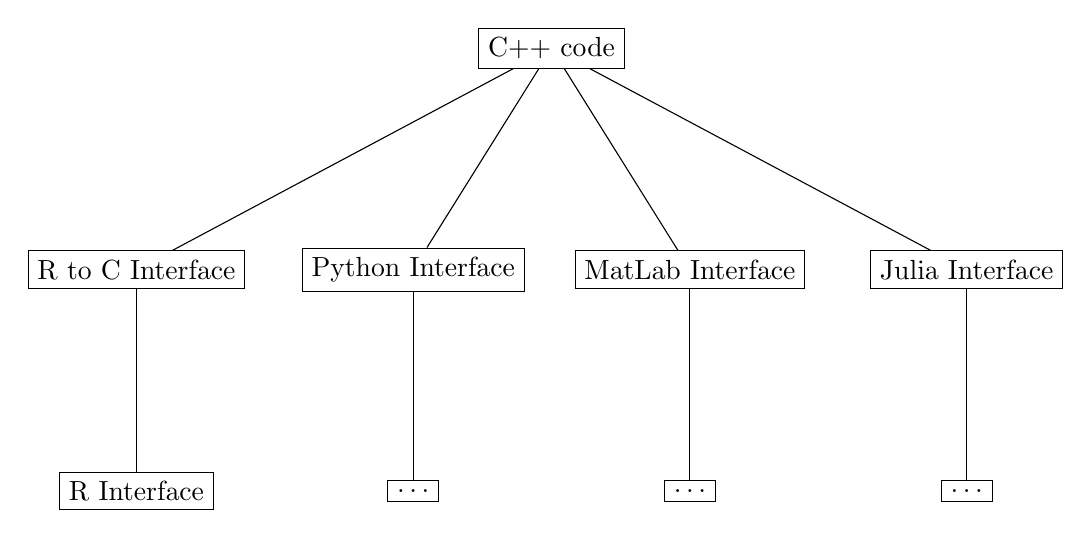
\begin{tikzpicture}[level distance=8em, sibling distance=10em,
  every node/.style = {shape=rectangle, draw, align=center}]]
  \node {C++ code}
    child { node {R to C Interface} 
      child { node {R Interface} }
    }
    child { node {Python Interface} 
      child { node {$\ldots$} }
    }
    child { node {MatLab Interface} 
      child { node {$\ldots$} }
    }
    child { node {Julia Interface} 
      child { node {$\ldots$} }
    };
\end{tikzpicture}

%%%
% Slide 8
%%%
\newpage
\section*{Penalized Regression on Steroids}

Installation: 

\begin{verbatim}
> devtools::install_github("austindavidbrown/pros/R-package")
\end{verbatim}

A single fit function with prediction

\begin{verbatim}
> fit <- pros(X, y, alpha, lambda)
> predict(fit, new_X)
\end{verbatim}

A cross-validation fit function with prediction

\begin{verbatim}
> cv <- cv.pros(X, y, alpha)
> predict(cv, new_X)
\end{verbatim}

There is even a \href{https://github.com/austindavidbrown/pros/blob/master/R-package/pros.pdf}{reference manual}.

\vspace{.5cm}
Yes, I know the name is bad.

%%%
% Slide
%%%
\newpage
\section*{The Boston Housing Dataset Analysis}

The Boston Housing dataset is popular from Harrison et al. \cite{boston_housing}.
There are 13 predictors and the response is the median value of owner-occupied homes in \$1000s.

\begin{itemize}
\item The data is randomly split into a training set with 404 observations and a test set with 102 observations.

\item The predictor data is standardized.

\item Basic 10-fold cross-validation and no special tuning.

\item The \textbf{glmnet} \cite{glmnet} library was used for the Lasso and the ElasticNet.

\item \textbf{pros} \cite{pros} was used to fit the new penalty.

\item The random seed was set to 8989.

\item The code is available to you at the \textbf{pros} repository \cite{pros}.
\end{itemize}

%%%
% Slide
%%%
\newpage
\section*{The Boston Housing Dataset Results}

\begin{center}
\begingroup
\setlength{\tabcolsep}{6pt} % Default value: 6pt
\renewcommand{\arraystretch}{2} % Default value: 1
\begin{tabular}{ l l l}
\textbf{Penalty} & \textbf{Tuning} & \textbf{Test MSE} \\
Lasso Penalty (glmnet) & $\alpha = (1, 0)$ & 28.52329 \\

ElasticNet Penalty (glmnet) & $\alpha = (1/2, 1/2)$  & 27.46224   \\

New Penalty (pros) & $\alpha = (1/2, 0, 1/2, 0, 0, 0)$ & 26.31973 \\

New Penalty (pros) & $\alpha = (1/2, 0, 0, 0, 0, 1/2)$ & 26.3852 \\

Tuned ElasticNet Penalty (glmnet) & $\alpha = (.25, .75)$  & 26.80933   \\

New Penalty (pros) & $\alpha = (.25, 0, .75, 0, 0, 0)$ & 26.25065 \\

Tuned New Penalty (pros) & $\alpha = (.1, 0, .9, 0, 0, 0)$ & 26.21775 \\
\end{tabular}
\endgroup
\end{center}


%%%
% Slide
%%%
\newpage
\section*{The Boston Housing Dataset Notes}

\begin{itemize}
\item The un-tuned 4th moment Penalty and un-tuned Elasticnet both removed age, but have different solutions otherwise.

\item The 10th moment penalty produces no sparsity.
\end{itemize}

%%%
% Slide
%%%
\newpage
\section*{The Prostate Cancer Dataset Analysis}

This is a popular dataset from Stamey et al. \cite{prostate} and analyzed in the ElasticNet paper by Zou and Hastie \cite{elasticnet}.
There are 8 predictors and the response is the log of the prostate specific antigen.

\begin{itemize}
\item The data is split into a training set with 67 observations and a test set with 30 observations.

\item The predictor data is standardized.

\item The \textbf{glmnet} \cite{glmnet} library was used to fit and tune the Lasso and a naive ElasticNet.

\item \textbf{pros} \cite{pros} was used to fit the new penalty.

\item 10-fold cross-validation and crude manual tuning were used.

\item The random seed was set to 8989.

\item The code is available to you at the \textbf{pros} repository \cite{pros}.

\end{itemize}

%%%
% Slide
%%%
\newpage
\section*{The Prostate Cancer Dataset Results}

\begin{center}
\begingroup
\setlength{\tabcolsep}{1pt} % Default value: 6pt
\renewcommand{\arraystretch}{2} % Default value: 1
\begin{tabular}{ l l l}
\textbf{Penalty} & \textbf{Tuning} & \textbf{Test MSE} \\
Lasso Penalty (glmnet) & $\alpha = (1, 0)$ & 0.4443432-0.4646501 \\
"Tuned" ElasticNet Penalty (glmnet) & $\alpha = (1/2, 1/2)$  & 0.4539684-0.4554527   \\
ElasticNet (pros) & $\alpha = (1/2, 1/2, 0, 0, 0, 0)$ & 0.5255658 \\
New Penalty (pros) & $\alpha = (1/2, 0, 1/2, 0, 0, 0)$ & 0.526071 \\
New Penalty (pros) & $\alpha = (1/2, 1/4, 1/4, 0, 0, 0)$ & 0.5256688 \\
\end{tabular}
\endgroup
\end{center}

%%%
% Slide
%%%
\newpage
\section*{The Prostate Cancer Dataset Results}

\begin{itemize}
\item Seems Elasticnet \cite{elasticnet} is better for this dataset.

\item I am very confused as to why my results don't match and why glmnet gives varying results.

\item I think it should preform similar. However, the solutions do have different sparsity, which is interesting.

\item With manual tuning I do way better, which is strange. Maybe my CV is wrong? Maybe I broke something when I changed the random number generator.

\end{itemize}

%%%
% Slide
%%%
\newpage
\section*{Conclusion}

\begin{itemize}
\item I think that there are many "good" solutions to real problems and we can get "statistics" on these solutions by imposing more norms on the feasible sets building upon the Elasticnet \cite{elasticnet} idea.

\item I would like to explore even more sparsity inducing penalizations such as

\[
\lambda P'(\beta) = \lambda \alpha_1 \norm{\beta}_1 + \lambda \alpha_2 \norm{\beta}_\infty 
\]

\[
\lambda P''(\beta) = \lambda \alpha_1 \norm{\beta}_1 + \lambda \sum_{k = 2}^{10} \alpha_k \norm{\beta}_{k}
\]

\end{itemize}

%%%
% Slide
%%%
\newpage
\section*{Things to Address}

\begin{itemize}

\item Currently, you have to tune a step size. I need to implement a fast line search. This is not too difficult actually just ran out of time.

\item Add logistic regression

\item Look into convergence analysis.

\item C++ offers many random number generators. I use the 64-bit Mersenne Twister by Matsumoto and Nishimura (2000).

\item minor bugs like overflow checking.

\item I think my Cross-Validation implementation can be sped up.

\item Optimize code to run faster maybe Fortran?

\end{itemize}

%
% Bib
%
\newpage
\small
\begin{thebibliography}{1}

\bibitem{boston_housing}
Harrison, D. and Rubinfeld, D.L. (1978) Hedonic prices and the
     demand for clean air.  J. Environ. Economics and Management 5,
     81-102.

\bibitem{prostate}
Stamey, T.A., Kabalin, J.N., McNeal, J.E., Johnstone, I.M., Freiha, F., Redwine, E.A. and Yang, N. (1989)
Prostate specific antigen in the diagnosis and treatment of adenocarcinoma of the prostate: II. radical prostatectomy treated patients, Journal of Urology 141(5), 1076–1083.

\bibitem{pros}
PROS. \href{https://github.com/austindavidbrown/pros}{github.com/austindavidbrown/pros}

\bibitem{boyd_proximalalgs}
Neal Parikh and Stephen Boyd. 2014. Proximal Algorithms. Found. Trends Optim. 1, 3 (January 2014), 127-239. DOI=10.1561/2400000003 http://dx.doi.org/10.1561/2400000003

\bibitem{wright_cd_algs}
Stephen J. Wright. 2015. Coordinate descent algorithms. Math. Program. 151, 1 (June 2015), 3-34. DOI=10.1007/s10107-015-0892-3 http://dx.doi.org/10.1007/s10107-015-0892-3

\bibitem{eigen}
Guennebaud, Gaël (2013). Eigen: A C++ linear algebra library (PDF). Eurographics/CGLibs.

\bibitem{glmnet}
Jerome Friedman, Trevor Hastie, Robert Tibshirani (2010). Regularization Paths for Generalized Linear Models via Coordinate Descent. Journal of Statistical Software, 33(1), 1-22. URL http://www.jstatsoft.org/v33/i01/.

\bibitem{elasticnet}
Zou, H. and Hastie, T. (2005). Regularization and variable selection via the elastic net. Journal of the Royal Statistical Society: Series B, 67, 301–320.

\bibitem{nesterov}
Yurii Nesterov. 2014. Introductory Lectures on Convex Optimization: A Basic Course (1 ed.). Springer Publishing Company, Incorporated.

\end{thebibliography}

\end{document}

